\section{Äquivalenzrelationen}
Äquivalenzrelationen sind homogene Relationen, die...
\begin{itemize}
    \item \textbf{reflexiv} $xRx$
    \item \textbf{symmetrisch} $xRy \Rightarrow yRx$
    \item \textbf{transitiv} $xRy \wedge yRz \Rightarrow xRz$
\end{itemize}
...sind.
\subsection{Beispiele}
\begin{itemize}
    \item Die Gleichheitsrelation auf einer beliebigen Menge ist eine
    Äquivalenzrelation.
    \item Die Relation $\equiv_n$ ist auf der Menge $\mathbb{Z}$ durch:
    \begin{align*}
        a \equiv_n b \Leftrightarrow n \text{ teilt } (a - b)  
    \end{align*}
    11 ist kongruent 5 modulo 3 ($\equiv_3$), da $11 : 3 = 3$  Rest  2 
    und $5 : 3 = 1$  Rest  2 ist und somit die beiden Reste gleich sind.
\end{itemize}
\subsection{Äquivalenzklassen}
Es sei $\sim$ eine Äquivalenzrelation auf einer Menge $A$. 
\begin{itemize}
    \item Für $a \in A$ ist
    \begin{align*}
        [a]_{\sim} \coloneqq \{x \in A \mid a \sim x\}
    \end{align*}
    die Äquivalenzklasse von $a$ bezüglich $\sim$ und beinhaltet alle Elemente von A, die zu a in Relation
    $\sim$ stehen.
    \item Jedes Element einer Äquivalenzklasse nennen wir einen
    Repräsentanten dieser Äquivalenzklasse.
    \item Die Faktormenge $\sfrac{A}{\sim}$ von A modulo $\sim$ ist die Menge aller Äquivalenzklassen:
    \begin{align*}
        \sfrac{A}{\sim} \coloneqq \{[a]_{R} \mid a \in A\}
    \end{align*}
\end{itemize}
\subsubsection{Eigenschaften}
Ist $\sim$ eine Relation auf A, dann sind folgende Aussagen äquivalent:
\begin{itemize}
    \item $a \sim b$
    \item $[a]_{\sim} = [b]_{\sim}$
    \item $[a]_{\sim} \cap [b]_{\sim} \neq \emptyset$
    \item $a \in [b]_{\sim}$
    \item $b \in [a]_{\sim}$
\end{itemize}
\section{Halbordnungen}
Eine Halbordnung ist eine\dots
\begin{itemize}
    \item \textbf{reflexive}
    \item \textbf{transitive}
    \item \textbf{antisymmetrische}
\end{itemize}
\dots Relation.
\subsection{Notation}
Im Kontext von Ordnungsrelationen wird die Notation $R = (G,A)$ meistens $A,G$ geschrieben.
\subsubsection{Beispiele}
\begin{itemize}
    \item Ist A eine beliebige Menge, dann ist $\mathcal{P}(A),\subseteq$ eine Halbordnung.
    \item Die "normalen" kleiner oder gleich Relationen $(A,\leq)$ mit $A=\mathbb{N,Z,Q,R}$ sind Halbordnungen.
\end{itemize}
\subsection{Hasse-Diagramme}
Das Hasse-Diagramm einer Halbordnung $(A, \preceq)$ ist eine
vereinfachte Darstellung des gerichteten Graphen von $(A, \preceq)$ und
wird wie folgt konstruiert.
\begin{itemize}
    \item Die Richtung eines Pfleies $a \rightarrow B$ für Elemte $a,b \in A$ wird 
    dadurch zum Ausdruck gebracht, dass sich der Knoten b oberhalb von a befindet.
    \item Pfeile zwischen zwei Punkten a, b werden gelöscht, wenn es ein
    c mit $a \preceq c \preceq b$
    \item Pfeile, die von einem Punkt auf denselben Punkt zeigen (Schleifen), werden weggelassen.
\end{itemize}
\subsubsection{Beispiel}
Halbordnung $(\mathcal{P}(\{a,b,c\}), \subseteq)$
\\\\
\begin{center}
    \begin{tikzpicture}
        \matrix (A) [matrix of nodes, row sep=1.2cm]
        {
            $\{a,b\}$ & $\{a,c\}$ & $\{b,c\}$ \\
            $\{a\}$ & $\{b\}$ & $\{c\}$ \\
            & $\emptyset$ \\
        };
        \path (A-1-1)--(A-1-2) node[above=1.2cm] (link) {$\{a,b,c\}$};
        
        \foreach \i in {1,...,3}
        \draw (link.south) -- (A-1-\i.north);
        \foreach \i/\j in {1/2, 3/2, 2/1, 1/1, 3/3, 2/3}
        \draw (A-1-\i.south)--(A-2-\j.north);
        \foreach \i/\j in {1/2, 2/2, 3/2}
        \draw (A-2-\i.south)--(A-3-\j.north);
    \end{tikzpicture}
\end{center}
Teilbeitskeitrelation auf der Menge aller Teiler von 28:\\\\
\begin{center}
    \begin{tikzpicture}
        \node (1) at (0,0) {$1$};
        \node (7) at (1,1) {$7$};
        \node (2) at (-1,1) {$2$};
        \node (14) at (0,2) {$14$};
        \node (28) at (-1,3) {$28$};
        \node (4) at (-2,2) {$4$};
        \draw (1) -- (2);
        \draw (1) -- (7);
        \draw (2) -- (4);
        \draw (2) -- (14);
        \draw (7) -- (14);
        \draw (14) -- (28);
        \draw (4) -- (28);
    \end{tikzpicture}
\end{center}
\subsection{Spezielle Elemente}
Es sein $(A, \preceq)$ eine Halbordnung und $ X \subseteq A$. Ein Element $x \in X$ heisst (bezüglich $\preceq$):
\begin{itemize}
    \item minmales Element von X, falls:
    \begin{align*}
        \forall{y} \in X(y \preceq x \Rightarrow y = x)
    \end{align*}
    \item kleinstes Element von X, falls:
    \begin{align*}
        \forall{y} \in X(x \preceq y)
    \end{align*}
    \item maximals Element von X, falls:
    \begin{align*}
        \forall{y} \in X(y \preceq x \Rightarrow y = x)
    \end{align*}
    \item grösstes Element von X, falls:
    \begin{align*}
        \forall{y} \in X(x \preceq y)
    \end{align*}
\end{itemize}
\subsubsection{Beispiel}
Es sei die Halbordnung $\preceq$ gemäss dem untenstehenden gerichteten
Graph gegeben. Es gilt:
\begin{itemize}
    \item maximale Elemente: $d,e$
    \item grösste Elemente: keine
    \item minimale Elemente: $a$
    \item kleinste Elemente: $a$
\end{itemize}
\begin{center}
    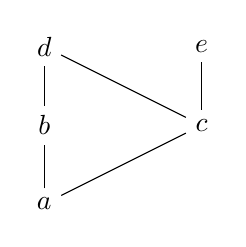
\begin{tikzpicture}
        \node (a) at (0,0) {$a$};
        \node (b) at (0,1) {$b$};
        \node (c) at (2,1) {$c$};
        \node (d) at (0,2) {$d$};
        \node (e) at (2,2) {$e$};
        \draw (a) -- (c);
        \draw (a) -- (b);
        \draw (b) -- (d);
        \draw (c) -- (d);
        \draw (c) -- (e);
    \end{tikzpicture}
\end{center}
\subsubsection{im Gerichteten Graph}
\begin{itemize}
    \item Maximale Elemente entsprechen den Knoten im gerichteten
    Graph von denen keine Pfeile weg zeigen (ausser Schleifen).
    \item Grösste Elemente entsprechen den Knoten im gerichteten
    Graph zu denen von jedem Knoten ein Pfeil hin zeigt.
    \item Minimale Elemente entsprechen den Knoten im gerichteten
    Graph zu denen keine Pfeile hin zeigen (ausser Schleifen).
    \item Kleinste Elemente entsprechen den Knoten im gerichteten
    Graph von denen zu jedem Knoten ein Pfeil zeigt.
\end{itemize}

